%



\dcs
We report on an experience related to an online video generator. 
% Some details have been reported in. % (\url{http://bref30ans.canalplus.fr}). 
 Compared to~\cite{BrefVamos14}, we add here further details under the angle of software protection.
% The goal is to explain that the video service is representative of the product line issues identified in the introduction; it acts as a case study~\cite{yin2002}.
% (i.e., "an empirical inquiry that investigates a contemporary phenomenon within its real-life context"~\cite{yin2002}).
 The service offers to generate variants of an humorous video. Internet users simply have to type their name, select 3 options, and a particular video is launched and visualised in the browser. % (see Figure~\ref{fig:brefo}, page~\pageref{fig:brefo}). 
The service is quite popular and successful: more than 1.7M of video variants have been generated in 1 week. 
%We had an interest in the Web site, since the service claims that a particular video is resulting from a combination among billions. Moreover the term % \emph{generator} is explicitly employed.  
% Our original intuition was that the video service resembles to a software product line, i.e., generative techniques and variability are likely to be present. 
 We put ourselves as attackers. We audited and studied the generator as a black box system without access to the source code of the server side. 
% Moreover, client side code is obfuscated as in the original service. 
%A first step was to reverse engineer the system. 
% In essence, reverse engineering \emph{"consists in deriving information from the available software artifacts and translating it into abstract representations more easily understandable by humans"}~\cite{canfora2011}. 
 We started reverse engineering the service through the analysis of the communications between the server and the client. 
Though the JavaScript was \emph{obfuscated}, the observations of HTTP requests and the use of a JavaScript debugger reveal the overall behaviour. We quickly noticed that all video variants are constituted of 18 sequences of videos that are themselves separated in several sub-parts. 
That is, a video variant is modularized. 


% \vspace*{-2mm}

The partitioning of the video in 18 sequences forms a first level of modularity (see \ding{192} in Figure~\ref{fig:generator}). % The objective is to avoid the generation of billions of videos on the server side.
For each sequence of a video, numerous alternatives are possible. This corresponds to a second level of modularity which focus on the variability of the video sequences (see \ding{193} in Figure~\ref{fig:generator}). A video variant results of the selection of an alternative for each sequence. The generator automatically selects an alternative, either based on the 3 selected options or through probabilistic choices for the other 15 sequences. 
% (the inference of frequencies per alternatives is out of the scope of the paper).
 Finally, a third level of modularity is realized by the partitioning of each alternative (see \ding{194} in Figure~\ref{fig:generator}). Overall modularity allows the server to share small video files and thus to improve the scalability/reactivity the service.
 
 
\begin{figure}
\centering
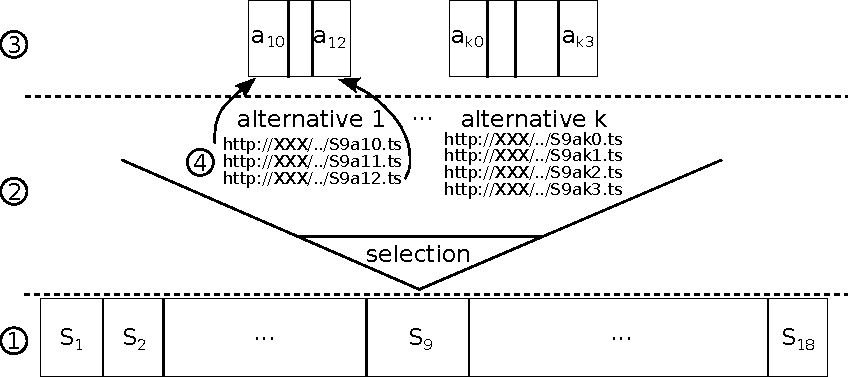
\includegraphics[width=1\linewidth]{figures/bref-generator.pdf}
\vspace*{-4mm}
\caption{\label{fig:generator}Video generator: modularity and variants}
% \vspace*{-4mm}
\end{figure}

Figure~\ref{fig:process} shows how the client and the server communicate to generate and play a video variant. First, the client asks for the generation of a new video. The server returns a list of file names corresponding to the selected sequences ($\{S1a2, ..., S18a4\}$ in our example).  
Each file corresponds to a playlist that defines the sub-parts of the sequence \eg in \ding{195} of Figure~\ref{fig:generator} the playlist defines 3 sub-videos: S9a10, S9a11 and S9a12.
The client downloads all the playlists and their corresponding videos. Finally, the client \emph{merges} the videos of the playlists and plays the resulting video variant.


\begin{figure}
\centering
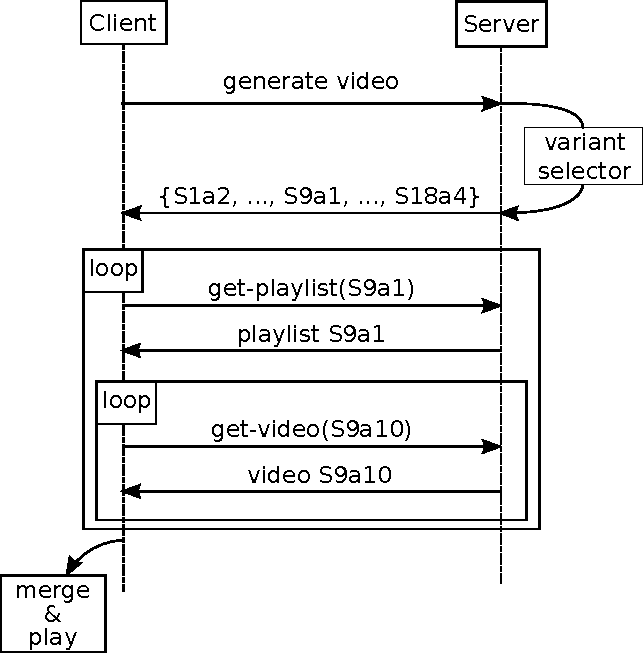
\includegraphics[width=0.7\linewidth]{figures/server-client.pdf}
\vspace*{-2mm}
\caption{\label{fig:process}Communications server/client}
\vspace*{-4mm}
\end{figure}





% We have then contacted the creators of the video generator with two research questions and goals in mind: (1) can we \emph{automate} the extraction of variation points and configurations (video variants)? (2) can we re-engineer another generator and configurator? 
% The creators accepted to collaborate and provided us with an access to an offline version of the generator. However we did not have access to the source code % neither in the server side nor in the client side. Like this, we can study the generator as a black box system -- as it would be the case in reality -- but without disturbing the deployed Web generator (e.g., with hundreds of HTTP requests). 
% \ma{We can remove this one: 
% The interest for the creators was to audit their systems.
 % security mechanisms for avoiding or at least complicating our tasks.
%




%  and defensive mechanisms have to be considered. 

\wprv
%
%  Our first audit showed that a reverse engineering work can get access to all the video sequences. Furthermore, ,
   % (see~\cite{BrefVamos14} for more details). 
% 15 new variation points are now apparent, out of which 13 are configurable (i.e., exhibiting at least 2 alternatives). 
% For the 3 variation points also present in the original configurator, users can now explicitly choose the alternatives. 
 The implementation of the product line can cause two important threats. 
The first threat is that an attacker can download the video sequences, which are protected by copyright. As digital content is a key business value, protecting the access to data becomes a security problem. Without defensive mechanisms, an attacker can extract and generate all the possible video variants of the original service. 
%
 The second consequence is that a new configurator can be re-engineered and could "kill the original idea"~\cite{BrefVamos14}. Specifically we showed it is straightforward to re-engineer a new generator and configurator in which users configure in a fine-grained way the 18 variations points -- instead of only 3 in the original version.
That is, with a re-engineered solution, the surprise effect is limited when getting a new video variant. Instead, users can control, choose and visualize \emph{any} alternative (video sequence). The creators of the generator did not have this intention  -- they did not want to jeopardize their trade secrets.

% calling to consider security issues. % -- though the idea of  
% -- thus dramatically limiting the \emph{surprise} effect. 

 % In other words, they have taken a strategic decision for, on-purpose, delimiting the scope of variability and restraining the visibility of some variation points and alternatives. 

% Our experience shows that the scoping of variability (i.e., what is visible to users) is a strategic solution and, 
% Overall the generator is well engineered and modularity is the right way to do from a development perspective. 
% Modularity is also needed to scale: as further emphasized in the next section, it is technically difficult to pre-generate millions of video variants.   \ma{says something like "modularity" or "featurization" is advocated by SPLE}

An important lesson learned is that the \emph{modularity} of data (video variants) poses a problem from a protection perspective.  
From a software engineering and product line perspective, modularity is undeniably good and remains a standing goal of any project. However modularity can backfire: an attacker can too easily understand the generation process and the differences between alternative sequences. 
With modularity, the task of determining the number of sequences and identifying the alternatives corresponding to each sequence does not face any obstacles. Similarly the collection and the \emph{composition} of video sequences is immediately understood. 
% Overall, a malicious attacker could not only collect all videos but could also launch a new competing video generator service; it is not acceptable.

Another important lesson learned is that an attacker should have difficulties to navigate into the configuration space. Otherwise she will be able to understand the whole product line and extract trade secrets in a \emph{comprehensive} and \emph{automatic} manner. Protection mechanisms for blocking frequent requests are worth considering but may not be sufficient. 
% An attacker can have difficulties to explore the modularity space.

 
% \ma{insist more on the "configurations" problem; rephrase or insist more on the "variability" aspect}




\begin{figure*}
\centering
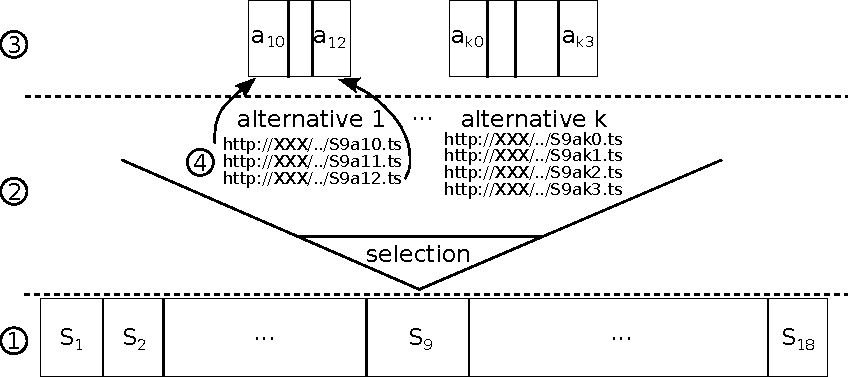
\includegraphics[width=0.6\linewidth]{figures/bref-generator.pdf}
\caption{\label{fig:generator}Video generator}
\end{figure*}

We report on an experience related to an online video generator. % (\url{http://bref30ans.canalplus.fr}). 
As we will see, the video service is quite representative of the "modularity problem" identified in the introduction; it acts as a case study~\cite{yin2002}.
% (i.e., "an empirical inquiry that investigates a contemporary phenomenon within its real-life context"~\cite{yin2002}).

The service offers to generate variants of an humorous video. Internet users simply have to type their name, select 3 options, and a particular video is launched and visualised in the browser. % (see Figure~\ref{fig:brefo}, page~\pageref{fig:brefo}). 
The service is quite popular and successful: more than 1.7M of video variants have been generated in 1 week. 
%We had an interest in the Web site, since the service claims that a particular video is resulting from a combination among billions. Moreover the term % \emph{generator} is explicitly employed.  
% Our original intuition was that the video service resembles to a software product line, i.e., generative techniques and variability are likely to be present. 
 We put ourselves as attackers. We audit and studied the generator as a black box system without access to the source code of the server side. 
% Moreover, client side code is obfuscated as in the original service. 

%A first step was to reverse engineer the system. 
% In essence, reverse engineering \emph{"consists in deriving information from the available software artifacts and translating it into abstract representations more easily understandable by humans"}~\cite{canfora2011}. 
We start reverse engineering the service through the analysis of the communications between the server and the client. 
Though the JavaScript was obfuscated, the observations of HTTP requests and the use of a JavaScript debugger reveal the overall behaviour. We quickly noticed that all video variants are constituted of 18 sequences of videos that are themselves separated in several sub-parts. 
That is, a video variant is modularized. 


The partitioning of the video in 18 sequences forms a first level of modularity (see \ding{192} in Figure~\ref{fig:generator}). The objective is to avoid the generation of billions of videos on the server side.
For each sequence of a video, numerous alternatives are possible. This corresponds to a second level of modularity which focus on the variability of the video sequences (see \ding{193} in Figure~\ref{fig:generator}). A video variant results of the selection of an alternative for each sequence. The generator automatically selects an alternative, either based on the 3 selected options or through probabilistic choices for the other 15 sequences. (The inference of frequencies per alternatives is out of the scope of the paper).
Finally, a third level of modularity is realized by the partitioning of each alternative (see \ding{194} in Figure~\ref{fig:generator}). This allows the server to share small video files in order to improve the scalability and the reactivity of the service.



Figure~\ref{fig:process} shows how the client and the server communicate to generate and play a video variant. First, the client asks for the generation of a new video. The server selects a video variant and returns a list of file names corresponding to the selected sequences ($\{S1a2, ..., S18a4\}$ in our example).  
Each file corresponds to a playlist that defines the sub-parts of the sequence. For example, the playlist named \textit{S9a1} defines 3 sub-videos: S9a10, S9a11 and S9a12 (see \ding{195} in Figure~\ref{fig:generator}).
The client downloads all the playlists and their corresponding videos. Finally, the client \emph{merges} the videos of the playlist and plays the resulting video variant.


\begin{figure}
\centering
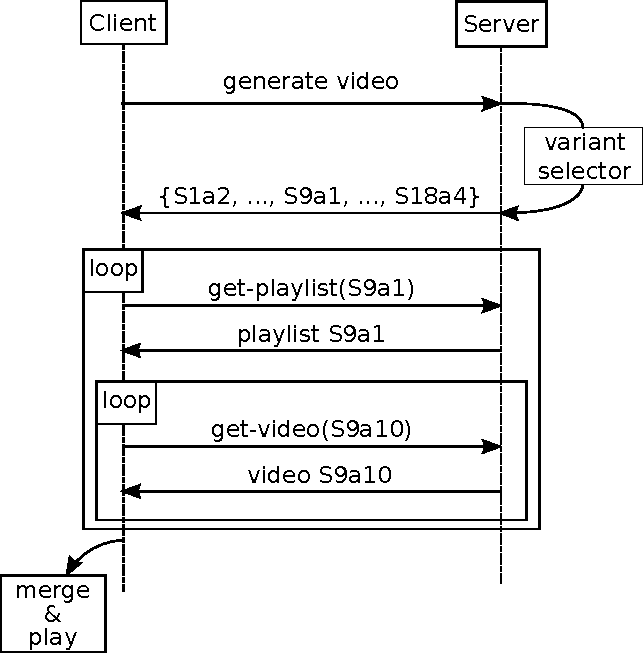
\includegraphics[width=0.9\linewidth]{figures/server-client.pdf}
\caption{\label{fig:process}Communications between server and client}
\end{figure}





% We have then contacted the creators of the video generator with two research questions and goals in mind: (1) can we \emph{automate} the extraction of variation points and configurations (video variants)? (2) can we re-engineer another generator and configurator? 
% The creators accepted to collaborate and provided us with an access to an offline version of the generator. However we did not have access to the source code % neither in the server side nor in the client side. Like this, we can study the generator as a black box system -- as it would be the case in reality -- but without disturbing the deployed Web generator (e.g., with hundreds of HTTP requests). 
% \ma{We can remove this one: 
% The interest for the creators was to audit their systems.
 % security mechanisms for avoiding or at least complicating our tasks.
%



The reverse engineering work have allowed us to download all the video sequences and re-engineer a new generator and configurator. This time, users can configure in a fine-grained way the 18 variations points -- instead of only 3 in the original version (see~\cite{BrefVamos14} for more details). 
% 15 new variation points are now apparent, out of which 13 are configurable (i.e., exhibiting at least 2 alternatives). 
% For the 3 variation points also present in the original configurator, users can now explicitly choose the alternatives. 

Our reverse engineering work poses two important threats. 
First, we showed that an attacker is able to download the video sequences which are protected by copyright. As digital content is a key business value, protecting the access to data becomes a security problem. Without defensive mechanisms, an attacker can extract and generate all the possible video variants of the original service. 
Second, the new configurator could "kill the original idea". That is, with a re-engineered solution, the surprise effect is limited when getting a new video variant. Instead, users can control, choose and visualize \emph{any} alternative (video sequence). The creators of the generator did not have this intention, calling to consider security issues. % -- though the idea of  
% -- thus dramatically limiting the \emph{surprise} effect. 

 % In other words, they have taken a strategic decision for, on-purpose, delimiting the scope of variability and restraining the visibility of some variation points and alternatives. 

% Our experience shows that the scoping of variability (i.e., what is visible to users) is a strategic solution and, 
Overall the generator is well engineered and modularity is the right way to do from a development perspective. 
Modularity is also needed to scale: as further emphasized in the next section, it is technically difficult to pre-generate millions of video variants.   
However, an important lesson learned is that the modularity of data (video variants) also poses a problem from a security perspective.  
With modularity, an attacker can easily understand the generation process and the differences between alternative sequences. The task of determining the number of sequences and identifying the alternatives corresponding to each sequence does not face any obstacles. Similarly the collection and the re-combination of video sequences is immediate. Overall, a malicious attacker could not only collect all videos but could also launch a new competing video generator service; it is not acceptable.
%  and defensive mechanisms have to be considered. 



